%!TEX TS-program = xelatex
%!TEX encoding = UTF-8 Unicode
\documentclass{style/ntuthesis}
\usepackage{style/kcchang-ntuthesis}

% Using the tex-text mapping for ligatures etc.
\defaultfontfeatures{Ligatures=TeX, Mapping = tex-text}


%%%%%%%%%%%%%%%%%%%%%%%%%%%%%%%%%%%%%%%%%%%%%%%%%%%%%%%%%%%%%%%%%%%%%%%%%%%%%%
% Setting fonts
%%%%%%%%%%%%%%%%%%%%%%%%%%%%%%%%%%%%%%%%%%%%%%%%%%%%%%%%%%%%%%%%%%%%%%%%%%%%%%
% Mac system fonts
%\setmainfont{Times New Roman}
%\setsansfont[Scale = MatchLowercase]{Arial}
%\setmonofont[Scale = MatchLowercase]{Monaco}
%\setCJKmainfont[BoldFont = Songti TC Bold]{Songti TC Regular}
%%%%%%%%%%%%%%%%%%%%%%%%%%%%%%%%%%%%%%%%%%%%%%%%%%%%%%%%%%%%%%%%%%%%%%%%%%%%%%
% Windows system fonts
 \setmainfont{Times New Roman}
 \setsansfont[Scale = MatchLowercase]{Arial}
 \setmonofont[Scale = MatchLowercase]{Lucida Console}
 \setCJKmainfont{標楷體}
%%%%%%%%%%%%%%%%%%%%%%%%%%%%%%%%%%%%%%%%%%%%%%%%%%%%%%%%%%%%%%%%%%%%%%%%%%%%%%
% Linux system fonts
%\setmainfont{DejaVu Serif}
%\setsansfont[Scale = MatchLowercase]{DejaVu Sans}
%\setmonofont[Scale = MatchLowercase]{DejaVu Sans Mono}
%\setCJKmainfont{WenQuanYi Zen Hei}
%%%%%%%%%%%%%%%%%%%%%%%%%%%%%%%%%%%%%%%%%%%%%%%%%%%%%%%%%%%%%%%%%%%%%%%%%%%%%%
% Mercury Text, Latin Modern Sans, and Operator Mono Book (Non-system fonts
% \setmainfont{Mercury Text G1}
% \newfontfamily\rmnumeric{Mercury Numeric}
% \setsansfont[Scale = MatchLowercase]{Latin Modern Sans}
% \setmonofont[Scale = MatchLowercase]{Operator Mono Book}
% \setCJKmainfont[BoldFont = Songti TC Bold]{Songti TC Regular}
%%%%%%%%%%%%%%%%%%%%%%%%%%%%%%%%%%%%%%%%%%%%%%%%%%%%%%%%%%%%%%%%%%%%%%%%%%%%%%
% Other Chinese fonts
%\setCJKmainfont{cwTeX Q Ming}
%\setCJKmainfont{cwTeX Q Kai}
%%%%%%%%%%%%%%%%%%%%%%%%%%%%%%%%%%%%%%%%%%%%%%%%%%%%%%%%%%%%%%%%%%%%%%%%%%%%%%

\ifdefined\withwatermark
\CenterWallPaper{0.174}{watermark.pdf}
\setlength{\wpXoffset}{6.1725cm}
\setlength{\wpYoffset}{10.5225cm}
\fi


%%%%%%%%%%%%%%%%%%%%%%%%%%%%%%%%%%%%%%%%%%%%%%%%%%%%%%%%%%%%%%%%%%%%%%%%%%%%%%%%%%%%%%%%%%%%%%%
%%%%%%%%%%%%%%%%%%%%%%%%%%%%%%%%%%中文版新增部分%%%%%%%%%%%%%%%%%%%%%%%%%%%%%%%%%%%%%%%%%%%%%%%
%%%%%%%%%%%%%%%%%%%%%%%%%%%%%%%%%%%%%%%%%%%%%%%%%%%%%%%%%%%%%%%%%%%%%%%%%%%%%%%%%%%%%%%%%%%%%%%
\usepackage{titlesec}  %% 更改章節圖表的中文
\usepackage{titletoc}  %% 更改章節圖表的中文
\usepackage{indentfirst}  %% 英文第一段沒indent,此package使第一段有indent

%將目錄標題中文化使用下列指令
\renewcommand\contentsname{目錄}
\renewcommand\listfigurename{圖目錄}
\renewcommand\listtablename{表目錄}
%要寫成表1.1 圖1.1的話需加入下列指令
\newcommand{\loflabel}{圖}
\newcommand{\lotlabel}{表}
\renewcommand{\tablename}{表}
\renewcommand{\figurename}{圖}
%%%%%%%%%%%%%%%%%%%%%%%%%%%%%%%%%%%%%%%%%%%%%%%%%%%%%%%%%%%%%%%%%%%%%%%%%%%%%%%%%%%%%%%%%%%%%%%
%%%%%%%%%%%%%%%%%%%%%%%%%%%%%%%%%%中文版新增部分%%%%%%%%%%%%%%%%%%%%%%%%%%%%%%%%%%%%%%%%%%%%%%%
%%%%%%%%%%%%%%%%%%%%%%%%%%%%%%%%%%%%%%%%%%%%%%%%%%%%%%%%%%%%%%%%%%%%%%%%%%%%%%%%%%%%%%%%%%%%%%%





% Your information goes here
%!TEX root = "../thesis.tex"
% author: Tz-Huan Huang [http://www.csie.ntu.edu.tw/~tzhuan]

% ----------------------------------------------------------------------------
% "THE CHOCOLATE-WARE LICENSE":
% Tz-Huan Huang wrote this file. As long as you retain this notice you
% can do whatever you want with this stuff. If we meet some day, and you think
% this stuff is worth it, you can buy me a chocolate in return Tz-Huan Huang
% ----------------------------------------------------------------------------

% Syntax: \var{English}{Chinese}
\university{National Taiwan University}{國立臺灣大學}
\college{College of Social Sciences}{社會科學院}
\institute{Department of Economics}{經濟學系}
\title{Practical Defensive Magic and Its Use Against the Dark Arts}{實用防禦魔法及其對抗黑魔法之使用}
\author{Harry James Potter}{哈利·詹姆·波特}
\studentid{R12345678}
\advisor{Albus Dumbledore, Ph.D.\\ Minerva Mcgonagall, Ph.D.}{鄧不利多{ }博士、麥米奈娃{ }博士}
\defenseyear{2017}{106}
\defensemonth{July}{7}
\defenseday{24}

\begin{document}

\frontmatter

\makecover

\makecertification
%\includepdf[pages={1}]{.pdf}
% 中文版新增部分 use scanned certification 
\setlength{\parindent}{2em}
% 中文版新增部分,設置第一段的縮排長度


\begin{acknowledgementszh}
\noindent 「勇氣有很多種」鄧不利多笑著說道。
「我們需要非常大的勇氣,才能站起來反抗我們的敵人;
但要反抗我們的朋友,同樣也需要非凡的勇氣才能做到。」\\
---《哈利波特:神秘的魔法石》
\end{acknowledgementszh}

\begin{acknowledgementsen}
\noindent ``There are all kinds of courage,'' said Dumbledore, smiling. 
``It takes a great deal of bravery to stand up to our enemies, 
but just as much to stand up to our friends.''
--- {\it Harry Potter and the Sorcerer's Stone}
\end{acknowledgementsen}
\begin{abstractzh}
\noindent 
世界不會分好人和壞人,每個人內心都有光明和黑暗,真正重要的是我們如何選擇,知道我們究竟是什麼人。
---《哈利波特:鳳凰會的密令》\\[10mm]
{\bf 關鍵詞:}黑魔法防禦術、正氣師、催狂魔、佛地魔。\\
{\bf JEL 分類代號:}D72、L82、D83、C81。
\end{abstractzh}

\begin{abstracten}
\noindent 
We've all got both light and dark inside us. 
What matters is the part we choose to act on. 
That's who we really are.
--- {\it Harry Potter and the Order of the Phoenix}\\[10mm]
{\bf Keywords:} Defense Against the Dark Arts, auror, dementor, Voldemort.\\
{\bf JEL Classification:} D72, L82, D83, C81.
\end{abstracten}



\tableofcontents
\renewcommand{\numberline}[1]{\loflabel~#1\hspace*{1em}}
% 中文版新增部分,圖1圖2
\listoffigures
\renewcommand{\numberline}[1]{\lotlabel~#1\hspace*{1em}}
% 中文版新增部分,表1表2
\listoftables

\mainmatter

\fontsize{12}{13}\selectfont
% Your thesis goes here
%\input{files/test}
\chapter{Introduction}
\label{c:intro}

\epigraph{
\fontsize{12}{13}\selectfont 
\it
It is our choices, Harry, that show what we truly are, 
far more than our abilities.
}
{
\fontsize{12}{16}\selectfont 
--- Albus Percival Wulfric Brian Dumbledore
}



This is an \XeLaTeX template for typesetting thesis in the social sciences in 
National Taiwan University. 
The original document is created by 
\href{https://github.com/tzhuan/ntu-thesis}{Tz-Huan Huang}. 
\href{https://github.com/KengChiChang/ntuthesis-socsci}{This version} 
is amended by 
\href{https://github.com/KengChiChang/ntuthesis-socsci}{Keng-Chi Chang}
to meet some conventions in the social sciences (especially economics)
and to improve the ease of editing and reading.~\footnote{
  If you find any problems or come up with any suggestions, 
  please feel free to email 
  \href{mailto:kengchi.chang.tw@gmail.com?subject=ntuthesis-socsci}{me}.
}

This template proceeds as follows: 
Section~\ref{s:citation} contains some citations.
Section~\ref{s:equation} shows some equations.
Section~\ref{s:table} imports a table.
Section~\ref{s:figure} includes a figure.
Section~\ref{s:todo} demonstrates the use of todo notes, and finally concludes.
\chapter{Literature Review}
\label{c:lit}

\section{Citation Example}
\label{s:citation}

This section showcases some citations under common scenarios.

\cite{bonica:ajps2014,donoho:wp2015,meyersson:e2014,akerlof:qje2000,bond:apsr2015,broockman:s2016,nunn:aer2011,gentzkow:2017,hastie:2009,chetty:2017,national-opinion-research-center:2017,pew-research-center:2016b,the-new-york-times:2016}.

\chapter{Model and Method}
\label{c:model&method}

\section{Equation Example}
\label{s:equation}

Here is Equation~\ref{eq:mle}.
\begin{align} \label{eq:mle}
\begin{split}
\mathcal{L}\left(\vec{\theta}, \vec{\phi}, \vec{\alpha}, \vec{\beta}, \gamma \,|\, \boldsymbol{\mathrm{y}}\right)&=\prod_{i\in\mathrm{user}}\prod_{j\in\mathrm{page}}\mathrm{logit}^{-1}\left(\pi_{ij}\right)^{y_{ij}}\left(1-\mathrm{logit}^{-1}\left(\pi_{ij}\right)\right)^{1-y_{ij}},\\
\left\{\hat{\vec{\theta}},\hat{\vec{\phi}}\right\}&=\argmax_{\vec{\theta}, \vec{\phi}}\,\mathcal{L}\left(\vec{\theta}, \vec{\phi}, \vec{\alpha}, \vec{\beta}, \gamma \,|\, \boldsymbol{\mathrm{y}}\right),
\end{split}
\end{align}
where $\pi_{ij}=\alpha_i+\beta_j-\gamma\left\lVert\theta_i-\phi_j\right\rVert^2$. 

\chapter{Data Processing and Results}
\label{c:data&result}

\section{Table Example}

Table~\ref{t:affiliation} is an affiliation matrix.

\begin{table}
\begin{center}
\begin{threeparttable}
\caption{Affiliation Matrix (Part)}
\label{t:affiliation}
\centering
\begin{tabular}{l*6{S[table-format=7.0]}}
  \toprule
  & {Trump} & {FoxNews} & {TeaParty} & {Clinton} & {CNN} & {NYTimes} \\ 
  \midrule
  Trump & 2243216 & 1078513 & 128225 & 32731 & 120963 & 25842 \\ 
  FoxNews & 1078513 & 2449174 & 148016 & 87084 & 186850 & 63401 \\ 
  TeaParty & 128225 & 148016 & 242089 & 1528 & 10738 & 2162 \\ 
  Clinton & 32731 & 87084 & 1528 & 1768980 & 351210 & 367021 \\ 
  CNN & 120963 & 186850 & 10738 & 351210 & 1201156 & 216163 \\ 
  NYTimes & 25842 & 63401 & 2162 & 367021 & 216163 & 986613 \\ 
  \bottomrule
\end{tabular}
\footnotesize 
{\it Notes}: 
Diagonal numbers are unique US users like at least one post of each pages, off-diagonal numbers are shared unique US users at least one post in both pages. 
Data ranges from 2015-01-01 to 2016-11-07. 
US users are defined by any user that at least reacted to any national politicians' (Sen, Rep, Gov) post once in 2015 and 2016.
\end{threeparttable}
\end{center}
\end{table}
\label{s:table}

\chapter{Validations}
\label{c:vali}

\section{Figure Example}
\label{s:figure}

Figure~\ref{f:media-score-cons} shows party affiliations of users on media fan pages against our estimate. 

\begin{figure}
\begin{center}
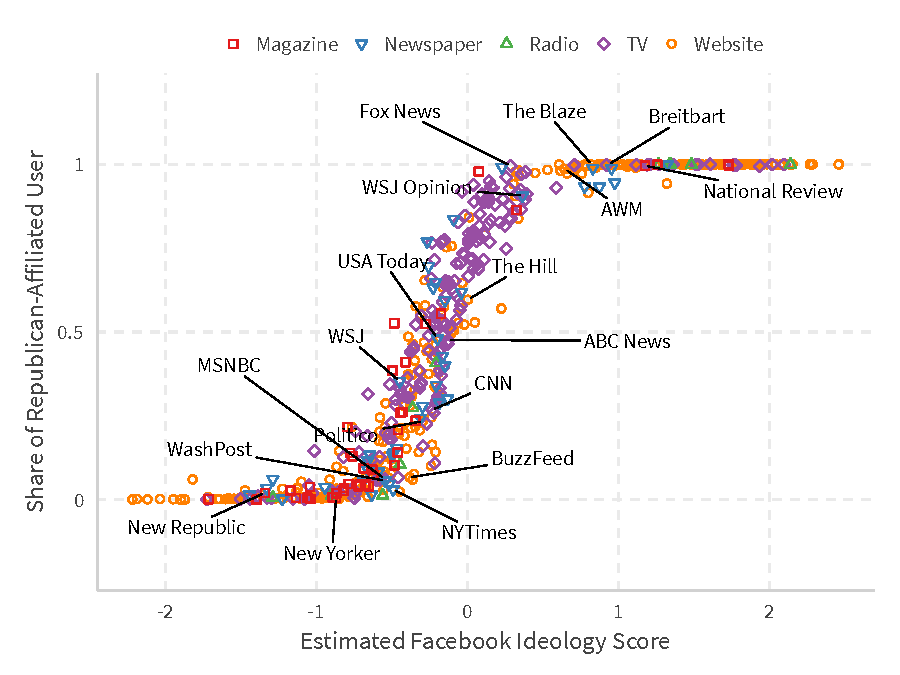
\includegraphics[width=\textwidth]{media-score-cons.pdf}
\caption{Validation of Media Slant}
\label{f:media-score-cons}
\floatfoot{{\it Notes}: 
A user is {\it Republican-affiliated} if their likes in all politicians are more for Republicans.
We only count user once a day on a page if they like more than one post on that day on that page.
We then sum all this kind of daily users up across each day.
Data ranges from 2015-01-01 to 2017-03-31.
}
\end{center}
\end{figure}

\chapter{Applications and Discussions}
\label{c:appli&disc}

\section{Todo Example}
\label{s:todo}

Hello, I'm Rita Skeeter!~\todo{Nonsense.}
I write for the Daily Prophet. 
But, of course, you know that, don't you? 
It's you we don't know. 
You're the juicy news.~\footnote{
  If you don't want to show a Todo List at the end of the document, 
  simply comment out the ``Todo List'' part in \texttt{thesis.tex}. 
  For more usage, please see the 
  \href{http://tug.ctan.org/macros/latex/contrib/todonotes/todonotes.pdf}{\textsf{todonotes}} 
  package.
}

\vspace{1em}

\missingfigure{Make a sketch of the Marauder's Map.}


\newpage
\phantomsection
%\addcontentsline{toc}{chapter}{\bibname}
\addcontentsline{toc}{chapter}{參考文獻} % 中文版新增部分,目錄有參考文獻四字
\renewcommand\bibname{參考文獻} % 中文版新增部分,正文中標題名為參考文獻

% Bibliography
\bibliographystyle{bib/thesis_style}
% Your bibliography goes here
\fontsize{12}{11}\selectfont
\Urlmuskip=0mu plus 1mu\relax % make bibliography tighter
\bibliography{bib/thesis}

\appendix
\addcontentsline{toc}{chapter}{附錄} % 中文版新增部分,目錄有附錄二字
\renewcommand\appendixname{附~錄} % 中文版新增部分,正文中標題名有附錄


\chapter{Further Results}
\label{c:further-result}

Dumbledore: ``It does not to do dwell on dreams, and forget to live.''


\chapter{Further Validations}
\label{c:further-vali}

Hermione: ``Me? Books and cleverness. There are more important things: friendship and bravery.''



\backmatter

% Todo List
% Comment the below two lines out if you don't want to list them in Contents
\addcontentsline{toc}{chapter}{Todo List}
\listoftodos[Todo List]

\end{document}

